%%%%%%%%%%%%%%%%%%%%%%%%%%%%%%%%%%%%%%%%%%%%%%%%%%%%%%%%%%%%%%%%%%%%%%
% LaTeX Example: Project Report
%
% Source: http://www.howtotex.com
%
% Feel free to distribute this example, but please keep the referral to
% howtotex.com Date: March 2011 
% 
%%%%%%%%%%%%%%%%%%%%%%%%%%%%%%%%%%%%%%%%%%%%%%%%%%%%%%%%%%%%%%%%%%%%%%
% How to use writeLaTeX: 
%
% You edit the source code here on the left, and the preview on the right shows
% you the result within a few seconds.
%
% Bookmark this page and share the URL with your co-authors. They can edit at
% the same time!
%
% You can upload figures, bibliographies, custom classes and styles using the
% files menu.
%
% If you're new to LaTeX, the wikibook is a great place to start:
    % http://en.wikibooks.org/wiki/LaTeX
%
%%%%%%%%%%%%%%%%%%%%%%%%%%%%%%%%%%%%%%%%%%%%%%%%%%%%%%%%%%%%%%%%%%%%%%

%%% Preamble
\documentclass[paper=a4, fontsize=8pt]{scrartcl} \usepackage[T1]{fontenc}
\usepackage[a4paper, total={6in, 8in}]{geometry}
\usepackage{fourier}

\usepackage[english]{babel}
% English language/hyphenation
\usepackage[protrusion=true,expansion=true]{microtype}
\usepackage{amsmath,amsfonts,amsthm} % Math packages
\usepackage{float}
\usepackage[pdftex]{graphicx}	\usepackage{url}
\usepackage{helvet}

%%% Custom sectioning
\usepackage{xcolor}
\usepackage{sectsty} 

\allsectionsfont{\normalfont}
\sectionfont{\color{cyan}}
\subsectionfont{\color{cyan}}


%%% Maketitle metadata
\newcommand{\horrule}[1]{\rule{\linewidth}{#1}} 	% Horizontal rule

\title{
		%\vspace{-1in} 	
		%\usefont{OT1}{bch}{b}{n}
		\huge Finding Single Crystal Peaks \\
}
\author{
		\normalfont 								\normalsize
        Samuel Jackson, Michael Hart, and \& Anders Markvardsen \\[-3pt]		\normalsize
        \today
}
\date{}


%%% Custom formatting 
\renewcommand{\baselinestretch}{1.5}
\renewcommand{\familydefault}{\sfdefault}
\setlength{\parindent}{0em}
\setlength{\parskip}{1em}

%%% Begin document
\begin{document} 
\maketitle

\section{Problem Statement} 
The WISH instrument runs approximately 60 single
crystal diffraction experiments a year. Identifying and correctly indexing
single crystal peaks in the diffraction pattern is the first step in the analysis
of a sample under study.  Identifying the location of both strong and weak
crystal peaks in the diffraction pattern allows the experimentalist to pin down
the orientation of the sample. The location, shape, and integration values of peaks is also central
to deducing structural information in subsequent analyses.

Unfortunately, finding peaks in a noisy background is a difficult problem.  A
significant proportion of instrument scientist and user time is spent adjusting
the output of the 3D peak finding algorithm in Mantid. The existing approach
focusses on identifying high density regions in the 3D Q (or if indexed, HKL) 
space of a particular run and uses a simple intensity \& density thresholding approach as the 
acceptance criteria for peak selection.

\begin{figure}[H]
\centering
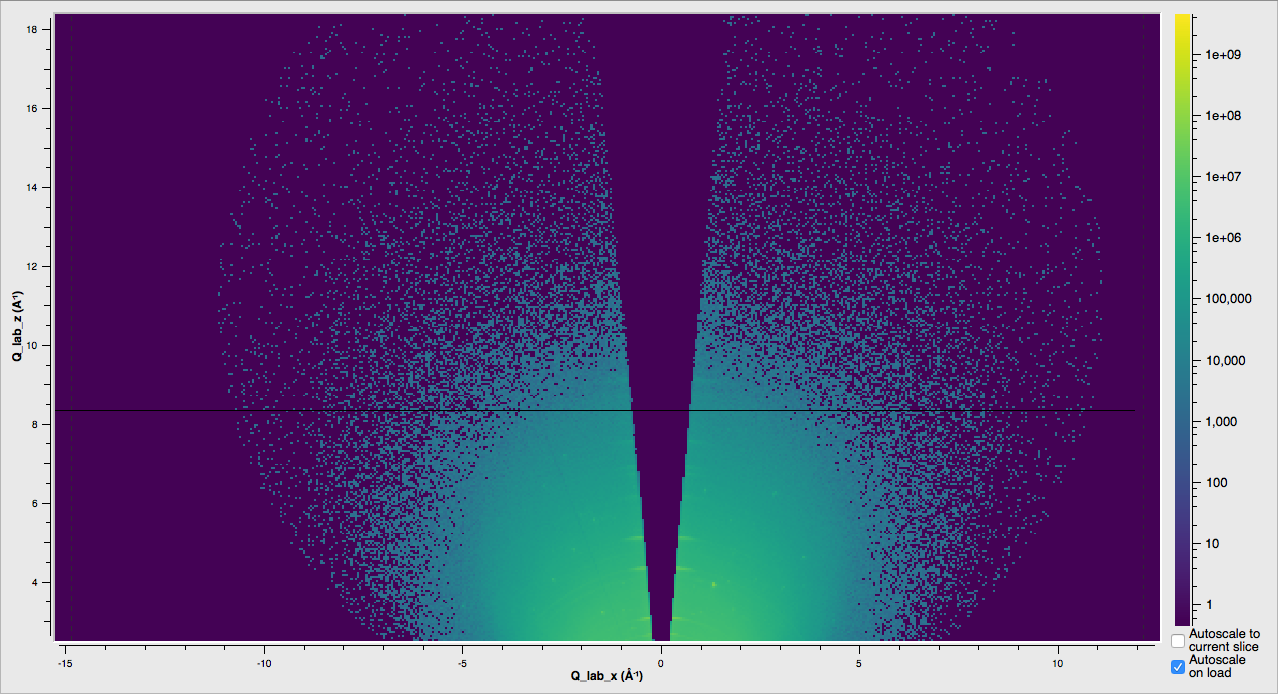
\includegraphics[width=0.7\textwidth]{WISH28145_4.png}
\caption{A slice through the $Q_y$ axis of WISH Q space}
\label{fig:wish-q-space}
\end{figure}

\begin{figure}[H]
\centering
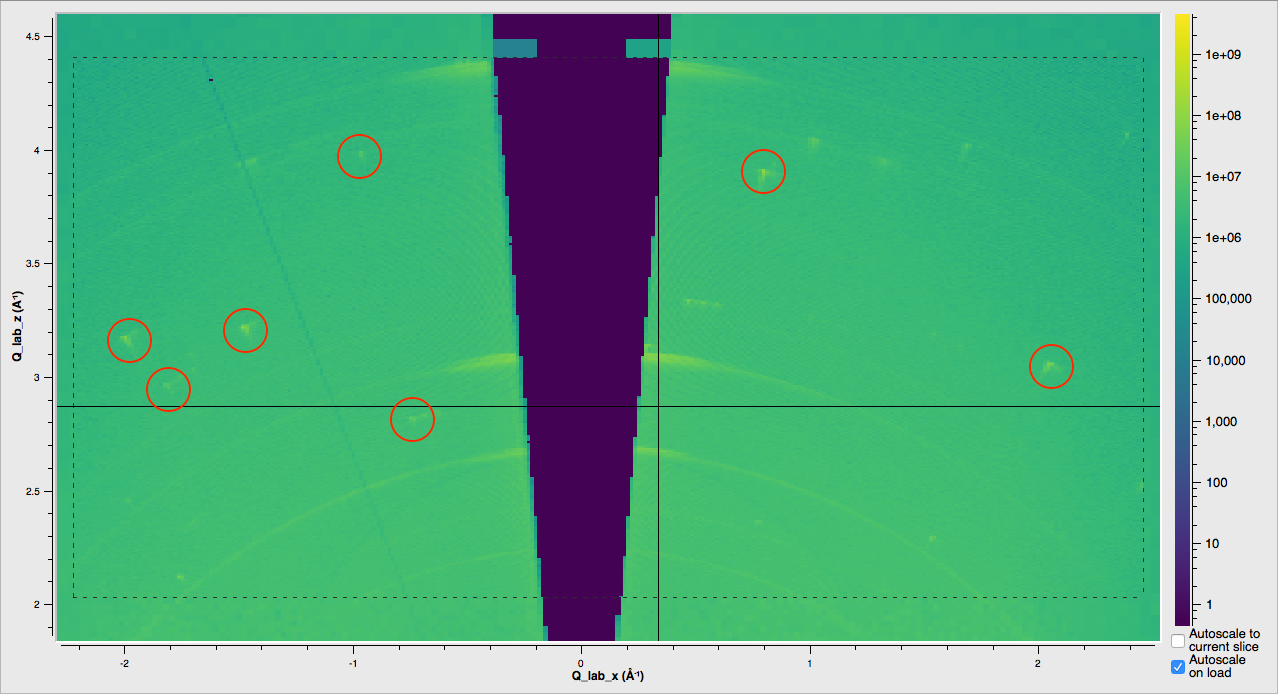
\includegraphics[width=0.7\textwidth]{WISH28145_2.png}
\caption{Single crystal diffraction Peaks in WISH Q space originating from the 
    sample. Also shown are powder diffraction
    rings which are typically generated by the sample container.}
\label{fig:wish-peaks}
\end{figure}

This approach frequently fails to produce adequate output for several reasons:
\begin{itemize}
\item False positive peaks. This is usually due to a combination 
of complicated background and artifacts in the diffraction pattern (such as 
powder diffraction rings).
\item False negative peaks. Usually weak peaks which are not detected by the 
algorithm due to noise or a threshold set too high to counter the background.
\item Double peaks, where two instances of the same peak are seen as two 
separate peaks.
\end{itemize}

Despite these complications, a human expert can easily visually identify peaks
in the pattern, providing motivation that machine learning techniques may have
more success where the existing approach fails.

\section{Automated Solutions} 
Ideally the process of identifying single crystal peaks should be as automated 
as possible, allowing scientists to focus on the more interesting analysis of 
their experiment. An ideal peak finder would likely have the following
properties:

\begin{itemize}
\item A low false positive \& false negative rate for both strong and weak
peaks.
\item A confidence estimate in the prediction. How certain is the algorithm that
this particular peak is a peak?
\item Information relating to the shape \& size of identified peak. Including
perhaps classification.
\item Continuous learning. The model should be able to take in corrections to
predicted results and use this to improve successful detection.
\end{itemize}

The following sections outline two approaches that could be taken as 
starting points to develop a machine learning solution to the problem in the 
previous section.

\subsection{Hand crafted features Approach}
One approach would be to use hand crafted features based on tried and tested
computer vision methods. Such an approach would most likely identify regions of
interest (ROIs) based on (for example) blob detection methods. An ROI detection
method could be build ontop of the existing peak detection method, but use the 
located points as the centre of an ROI. Discriminating 
features based on these ROIs, such as shape, intensity, or texture based metrics, 
can then be used to train a binary classification model. This could be any one of the 
commonly used models in machine learning such as a SVM or Random Forest. In fact 
it would be best to train a number of models on the same features and 
compare their performance. Classifiers such as these can easily be modified to 
give a confidence estimate on the predicted class. New images could then be 
shown to the trained system, the ROIs \& features calculated, and the ROIs with 
similar metrics would be predicted as containing a peak (or not).

An advantage of using this as a starting point is that such a system would
likely be much easier to develop and train. However, the performance of such a
system will be highly dependant on the method used to select ROIs and the choice of
features computed from those ROIs. Choosing this method would mean initially 
spending time investigating which methods will best suit the problem data.

\subsection{Neural Network based Approach}
Another approach would be to train a neural network directly on the data either
on the entire volume itself or on 2D slices (see section \ref{sec:data}). The 
architecture of the neural network would have to be explored experimentally, but 
the work in refs. \cite{wang2016x} and \cite{kiapour2014materials} on 
classifying x-ray data could provide a potential a starting point. 

An important point to consider when developing a neural network based approach is that this 
problem requires both object identification (``there are peaks'') and object 
detection (``the peaks are here''). Successful detection of where an object
is in an image is a computationally intensive problem, but recent work in the 
neural network community has produced some effcient solutions to mutliclass object detection problems
based on regression networks \cite{sermanet2013overfeat} and region proposal 
networks \cite{kiapour2014materials}, \cite{girshick2014rich}, \cite{renNIPS15fasterrcnn}.

\section{Datasets \& Representation}
\label{sec:data}
The current method for peak finding searches across 3D bins in the Q space of a 
particular run. Many domains which use the methods described in the preceeding section are applied 
directly to 2D images. For our problem we could either choose to develop a 
system which works directly on the 3D volume or slice the dataset
along a given axis to form a series of 2D images. The latter has the advantage 
of producing a large dataset set from only a few sample runs, with the 
caveat that some peak examples in adjacent slices would not necessarily be 
independent of one another. Ideally both methods should be investigated if time
and resources allow.

The other consideration with the representation is which space to use for
training and testing the model? Both will need to be the same for an apples to 
apples comparison. Q space seems the most logical here. Without necessarily 
knowing the orientation (UB) matrix in advance one cannot transform the data to HKL space. 
Using detector space would negate the problem of first having to convert the
data to Q (which is computationally slow) but has the disadvantage of being 
instrument specific and more difficult to relate adjacent spectra.

The lack of labelled data currently available is also an issue. Scientists
typically perform their peak identification on the fly during or after and experiment. There is
currently no single, consistently labelled ground truth dataset which can be
used. However, WISH scientists note that they do have some indexed peaks stored
which could possibly be used, but the extent and detail of the data is currenty unknown. 
This lack of data is a major sticking point for a machine 
learning approach. A good volume of diverse, labelled diffraction data is 
necessary for supervised learning methods. This is where being able to 
continuously learn from user input is likely to be useful. 


\begin{figure}[H]
\centering
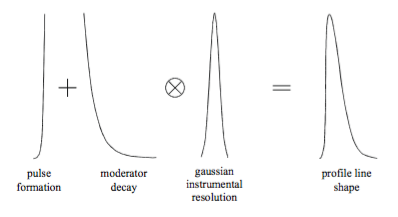
\includegraphics[width=0.7\textwidth]{peak-profile.png}
\caption{Components making up the peak line shape in time-of-flight diffraction.}
\label{fig:peak-profile}
\end{figure}

One way around this problem could be to use artificial or simulated data. Unlike 
many image analysis problems, it could be quite easy to simulate training
examples. Single crystal peaks at the most fundamental level be defined by the
instrument resolution function and functions for pulse formation and moderator
decay (see figure \ref{fig:peak-profile}). It should be relatively simple to 
generate data that closely resembles real experimental data using a combination of
know crystal lattices, instrument resolution, and a UB matrix. Another option is 
to use of software such as McStas 
\cite{McStas} or MCViNE \cite{MCViNE} could be used as starting points for 
generating datasets. How accurately simulated data would match features of real 
data has yet to be determined.

Another issue is that both the exisiting technique and the proposed versions above are 
limited as they can only incorporate visual data. More advanced 
methods which include heuristics based on, for example, the sample envrioment used could also 
possibly be incorporated. Modelling of this may be helpful to reduce
noise in the data, and this could easily be explored at the same time as attempting
to accuratly simulate TOF data.

\section{Implementation Considerations}
For initial development of the system the programming language Python would be
strongly recommended. This is for a number of reasons:

\begin{itemize}
\item Mantid, used for reducing the raw data, exposes a Python API.
\item Python is widely used in the scientific and machine learning communities.
\item Python has a wide variety of tried and tested image processing 
\cite{scikit-image} and machine learning \cite{scikit-learn} \cite{keras} 
libraries.
\item Python easily interoperates well with C/C++ meaning custom high 
performance functionality can easily be included.
\item Authors have familiarity with the language.
\end{itemize}

Additionally, there are some hardware considerations that must be addressed. 
WISH data is typically fairly large (~800Mb on disk, larger in memory) and the
transformation to Q space is computation intensive. This means that the any 
development machine need sufficient memory and processing power to handle these 
constraints. Furthermore, machine learning models, and in particular neural network models are typically also 
computationally expensive to train often requiring the use of GPUs for realistic 
training times. When larger computational resources are required, one option would be
to use the HPC resources maintained by STFC.

\section{Related Work}
We are unaware of any directly comparable work to the problem described here. 
The closest existing work found was that of refs.\cite{kiapour2014materials} and 
\cite{wang2016x} on the classification of x-ray scattering patterns using deep 
neural networks. While their work has some superficial similarities to this 
problem, it only classifies the pattern into a discrete category and says 
little about localisation of interesting artifacts used in the classification.

\section{Conclusion}
In conclusion, the problem of finding peaks in single crystal diffraction data 
has been outlined and the difficulties of the existing system have been listed.
Two feasible alternative approaches based on the machine learning paradigm have 
been presented. Based on the specification of the task at hand and its intersection
with similar challenges in the image processing \& machine learning communities
we feel that such a system would be feasible to build and could provide 
superior performance to the existing method. 

Based on the initial analysis of the problem we feel that the best option of the
two presented would be to use hand crafted features based on image 
processing techniques and a simple classification/regression learner. This has 
several advantages over the neural network option:

\begin{itemize}
    \item Implementation will likely be simpler, particularly with regard to peak localisation.
    \item Training will likely require less data.
    \item Single crystal peaks are relatively simple in apperance. A neural network would most likely be overkill for this specific problem.
\end{itemize}

However, it is worth emphasising that building such a system would not be without 
challenges. The major hurdles which we feel must be overcome are obtaining/creating 
enough labelled data for training and the computational expense of preprocessing 
WISH data to Q space during the training stage. 

Based on an initial analysis of this problem we feel that the next steps towards 
building an automated peak finding system in order of importance would be:

\begin{itemize}

\item Creation of ground truth dataset with a high variety of peak strengths \& shapes 
    from a multitude of representative samples. As mentioned previously the lack of good labelled
    data is a significant problem. We feel that due to the well defined and simplistic nature of 
    peaks our best option is to turn to simulating the data. Providing this is accurate to the 
    real data this would give us plenty of training examples to work with and also allow us
    to control the size of the data to make prototyping quicker \& easier.

\item Run the current peak finding method both on real experimental data and 
    on the simulated dataset and evalute the true \& false positive/negative rates achieved.
    This gives us a known baseline which we can use to measure the performance of subsequent
    prototypes against.

\item Develop a simple prototype system based on finding regions of interest in 
    slices from the q-space volume along a given axis and classifying regions as
    being a peak or not. At this point we would need to evaluate performance against
    the baseline. The prototype could then be improved and more complicated
    options explored based on performance against the baseline.

\end{itemize}

While it is easy to outline the next steps towards implementation, it is much more 
difficult to esimate the amount of time \& effort required, particularly for the 
third point above. To a certain extent decisions need to be made after experimenting
with the data and improving any models based on results and performance. All we can say
is that the three points above are perhaps the bare minimum steps required to get a simple
prototype potentially capable of out performing the exisitng method up and running.

This is to the best of our knowledge the first attempt at ISIS to use machine 
learning for improving data processing. We feel that machine learning has a lot to offer ISIS, 
and the success of this project will likely be the seed for further utilisation of such
techniques at ISIS, potentially greatly improving the quality and speed by which data
can be processed.

\bibliographystyle{plain}
\bibliography{sources} 
%%% End document
\end{document}
